% -*-LaTeX-*-

% $Log: fb-filters.tex,v $
% Revision 1.7  2007/12/25 17:47:12  stiber
% Some final cosmetic changes.
%
% Revision 1.6  2007/12/11 17:49:03  stiber
% Small changes to get ready for Witner 2008.
%
% Revision 1.5  2007/03/20 23:53:48  stiber
% Updated eqnarray to align.
%
% Revision 1.4  2007/03/20 18:14:34  stiber
% Modified for use as part of standalone text.
%
% Revision 1.3  2006/03/27 23:37:41  stiber
% Fixed errors in formulas; deleted end-of-chapter problem that lacked
% prerequisite material upon switching of textbook.
%
% Revision 1.2  2004/03/29 19:54:44  stiber
% Updated for Spring 2004 and new textbook (DSP First).
%
% Revision 1.1  2004/02/19 00:24:45  stiber
% Initial revision
%

\chapter{Feedback Filters}
\label{ch:fb-filters}

\section{Introduction}

In this chapter, we will continue to introduce filters, this chapter
focusing on \emph{feedback filters}, in which previous outputs are
combined with new inputs to produce new outputs. We will learn about
their structure, function, and the differences between feedforward and
feedback filters.  We will see that sometimes it is better to combine
these two kinds of filters. We will also briefly examine digital
filter design. After this chapter, you should understand important
concepts like the \emph{poles} (as compared to \emph{zeros}) of a
transfer function, \emph{impulse response}, and \emph{bandwidth}. You
should know about features of feedback filters and special types of
such filters, such as \emph{resons}.  You should be able to design
simple digital filters, implement them on a computer and use them to
solve some simple signal processing problems.

\subsection{Poles}

\begin{figure}
\centerline{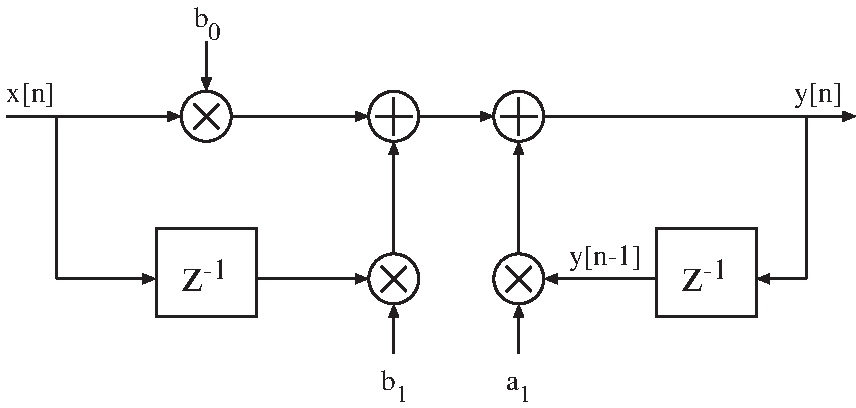
\includegraphics[width=0.5\textwidth]{ch-iir/fb-bdiag}}
\caption{Block diagram of a simple filter with both feedforward and
  feedback terms.\label{fig:fb-bdiag}}
\end{figure}

Figure~\ref{fig:fb-bdiag} presents the block diagram of a filter with
one feedforward and one feedback term; the feedback filter's signal
flowgraph is shown on the right. Compared to the feedforward one on
the left in the figure, we notice that instead of combining the input
signal with a delayed version, here the output signal is delayed and
``fed back'' to be combined with the input. The feedback processing
alone is expressed by
\begin{equation}
y[n] = x[n] + a_1 y[n-1]
\label{eq:fb-1p}
\end{equation}
(ignoring the factor of $b_0$) which is the equation for a simple
feedback filter with one delayed component. $a_1 y[n-1]$ is the
feedback term. You can see that the output at $n-1$ is used to compute
the output at time $n$. The combined filter's full defining equation
is
\begin{equation}
  y[n] = b_0 x[n] + b_1 x[n-1] + a_1 y[n-1]
  \label{eq:fb-ff}
\end{equation}
but for the moment we will concentrate on just the feedback.

From equation~(\ref{eq:fb-1p}), the z-transforms of the input and
output signals, and the delay operator $z^{-1}$, we can get the
filter's transfer function as follows:
\begin{align}
Y(z) &= X(z) + a_1z^{-1}Y(z) \notag\\
Y(z)[1-a_1z^{-1}] &= X(z) \notag\\
Y(z) &= \frac{1}{1-a_1z^{-1}}X(z)
\end{align}
Finally we have the transfer function:
\begin{align}
H(z) &= \frac{Y(z)}{X(z)} = \frac{1}{1-a_1z^{-1}} \notag \\
     &= \frac{z}{z-a_1} \label{eq:fb-xfer}
\end{align}
The magnitude response is:
\begin{equation}
|\mathcal{H}(\hat{\omega})|
  = |H(z)|
  = \left|\frac{z}{z-a_1}\right|=\left|\frac{1}{z-a_1}\right|
\label{eq:fb-1pmh}
\end{equation}
($|z|=1$ because we are only concerned with the magnitude when $z$ is
on the unit circle, and so its magnitude is always one).

\index{filter!poles|emph} The values of $z$ that make the denominator
of the transfer function zero (the roots of the denominator
polynomial, where the transfer function becomes infinite) are called
its \emph{poles}. In~(\ref{eq:fb-1pmh}), there is one pole at
$z=a_1$. In general, $a_1$ is not on the unit circle, and so the
phasor $z$ approaches it but is never equal to it.  Just as we did for
zeros, we can draw a line from the pole to the unit circle to indicate
the distance between $z$ and the pole.  However, now this distance is
in the denominator. Therefore, instead of $H(z)$ having a notch or dip
when $z$ nears a zero, it has a \emph{peak} when $z$ nears a pole.

\begin{figure}
\centerline{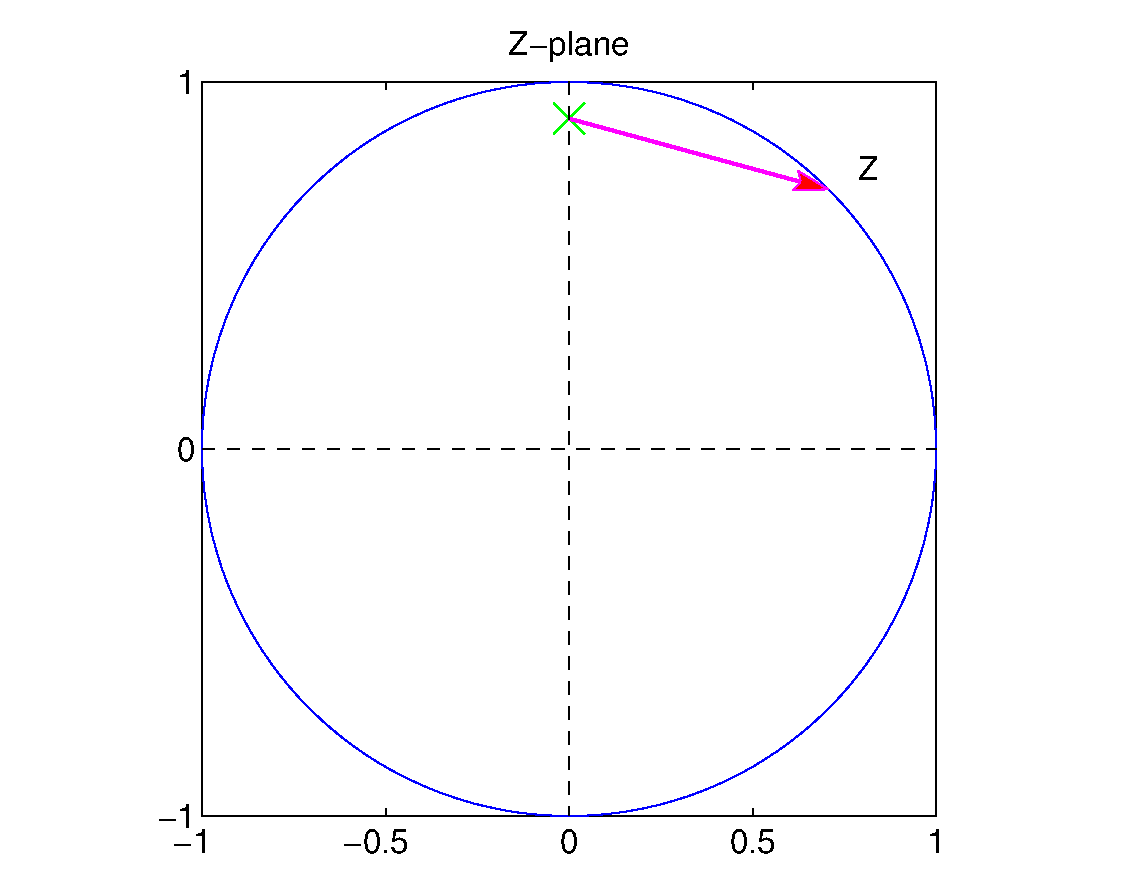
\includegraphics[height=3.5in]{ch-iir/fbexp_1p_c90}}
\caption{One pole in the $z$-plane, located at $r=0.9$ and
$\hat{\omega}_0=\pi/2$.\label{fig:fb-exp1pc90}}
\end{figure}

\begin{figure}
\centerline{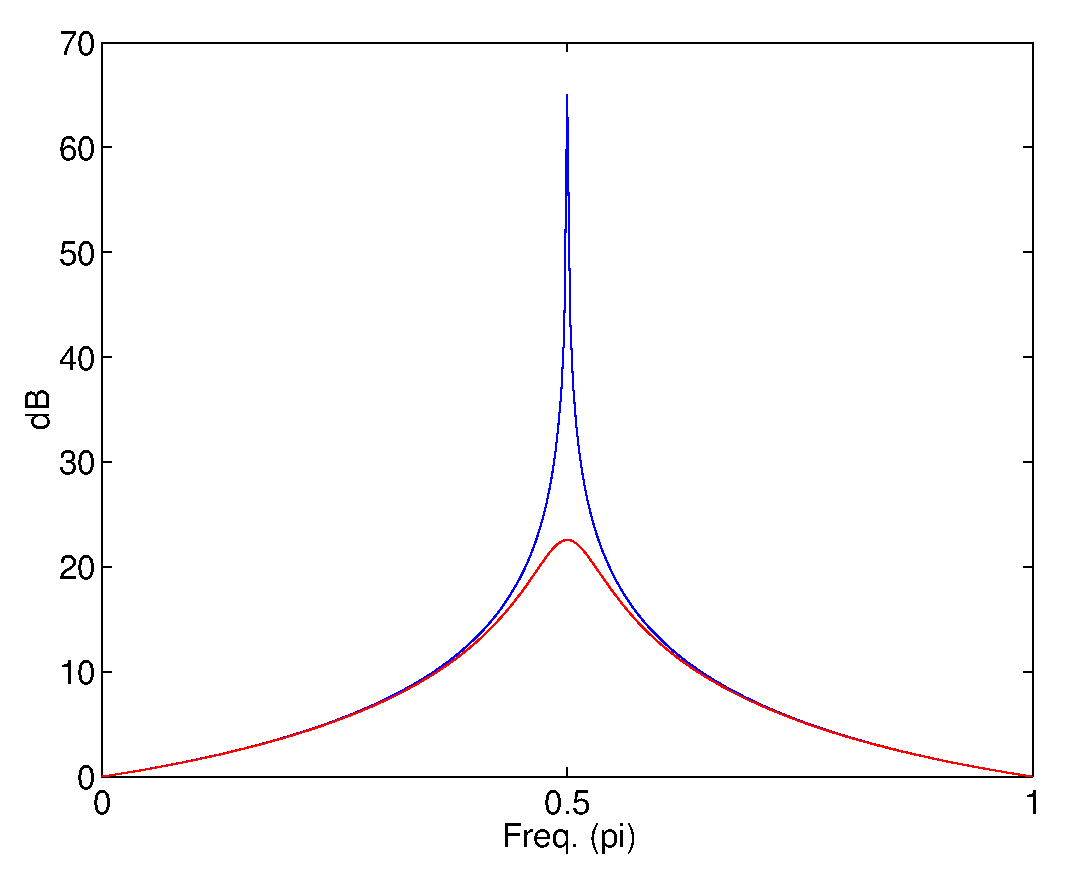
\includegraphics[height=3in]{ch-iir/fbexp_1p_h90_r1_r0-9}}
\caption[Magnitude response of two filters]{Magnitude response of two
  filters with poles located at $\hat{\omega}_0=\pi/2$ and $r=0.9$
  (bottom) or $r=1$ (top).\label{fig:fb-exp1ph90r2}}
\end{figure}

\paragraph*{Example~1} 
For the one pole filter~(\ref{eq:fb-1p}),
$a_1=re^{j\hat{\omega}_0}$. Figure~\ref{fig:fb-exp1pc90} shows this
pole when $r=0.9$ and
$\hat{\omega}_0=\pi/2$. Figure~\ref{fig:fb-exp1ph90r2} shows its
magnitude response. As expected, $|\mathcal{H}(\hat{\omega})|$ has a
``hill'' near $\hat{\omega}_0=\pi/2$. As $r$ moves closer to one, the
hill becomes steeper.

\subsection{Example: Computing Transfer Function and Impulse Response}

Compute the transfer function and impulse response of the system
described by the feedback filter, 
\begin{equation}
y[n] = 2x[n] + \frac{1}{2}y[n-1]
\end{equation}

By computing the z-transform of the both side of above equation and
using the fact that
\begin{equation}
y[n-1]\stackrel{\mathbf{Z}}{\longleftrightarrow} z^{-1}Y(z)
\end{equation}
we obtain,
\begin{equation}
Y(z)= 2X(z) + \frac{1}{2}z^{-1}Y(z).
\end{equation}
Hence the transfer function is 
\begin{equation}
H(z)= \frac{Y(z)}{X(z)} = \frac{2}{1-\frac{1}{2}z^{-1}}
    = \frac{2z}{z-\frac{1}{2}} \label{eq:fb-exxfer}
\end{equation}

$H(z)$ has a pole at $z=1/2$ and zero at $z=0$. Now we
compute its impulse response. Previously we had an example of an
exponential signal~(\ref{eq:zt-expof}) and its
z-transform~(\ref{eq:zt-expoF}), so we have
\begin{equation}
a^n\stackrel{\mathbf{Z}}{\longleftrightarrow}
\frac{1}{1-az^{-1}}, \quad n \ge 0, |z|>a
\end{equation}
This is of the same form as~(\ref{eq:fb-exxfer}), with $a=1/2$.  Using
this result, we obtain the inverse transform
\begin{equation}
h[n] = 2\left(\frac{1}{2}\right)^n, \quad n\ge 0 \label{eq:fb-eximp}
\end{equation}
where the left and right sides of equation~(\ref{eq:fb-eximp}) are the
inverse z-transforms of the left and right sides
of~(\ref{eq:fb-exxfer}).  This is the corresponding impulse response.

\subsection{Stability}

Let's examine equation~(\ref{eq:fb-1p}) again. Note that $y[n]$
doesn't only depend on $x[n]$. This means that, even if the input
signal is zero after some initial value, this feedback term can
continue to have a nonzero value and so the filter can still produce
some output. This is a major difference from feedforward filters,
where the output depends only on the input. As an extreme example,
consider the case where the input signal is a \emph{unit impulse},
\begin{equation}
x[n] = \delta[n] =
\left\{\begin{array}{rl}
1 & n=0\\
0  & n>0
\end{array}\right.
\end{equation}
which means it only has a value of one at the beginning, and then
turns off.  The output of any filter for a unit impulse is called,
logically enough, its \emph{impulse response}.  For the filter
in~(\ref{eq:fb-1p}) with coefficient $a_1=0.5$, the impulse response
is:
\begin{align}
y[0] &= x[0] = 1 \notag\\
y[1] &= x[1] + 0.5 y[0] = 0+0.5 \times 1 = 0.5 \notag\\
y[2] &= x[2] + 0.5 y[1] = 0+0.5 \times 0.5=0.25=0.5^2 \notag\\
y[3] &= x[3] + 0.5 y[2] = 0+0.5 \times 0.25=0.125=0.5^3 \notag\\
& \vdots  \notag \\
y[n] &= 0.5^n \label{eq:fb-1pexp}\\
& \vdots  \notag
\end{align}
You can see that the output $y[n]$ continues after $n=0$, but the
value becomes smaller each time, and will decay towards zero.  On the
other hand, if $a_1>1$, the output becomes bigger and bigger, and goes
to infinity. This second behavior is called \emph{unstable}.  From
equation~(\ref{eq:fb-1pmh}), we know that $a_1$ is a pole of the
filter.  In fact, a feedback filter with multiple poles $p_i$ is
stable if and only if
\begin{equation}
|p_i| < 1,  \text{ for all } i
\end{equation}
In other words, \emph{all} the poles must be inside the unit
circle. Here is the basic idea for a four-step (well,
three-step-and-a-note) proof of this:

\begin{enumerate}
\item \textbf{A feedback filter with $N$ feedback terms can be decomposed into
$N$ one-pole feedback filters.}

\begin{figure}
\centerline{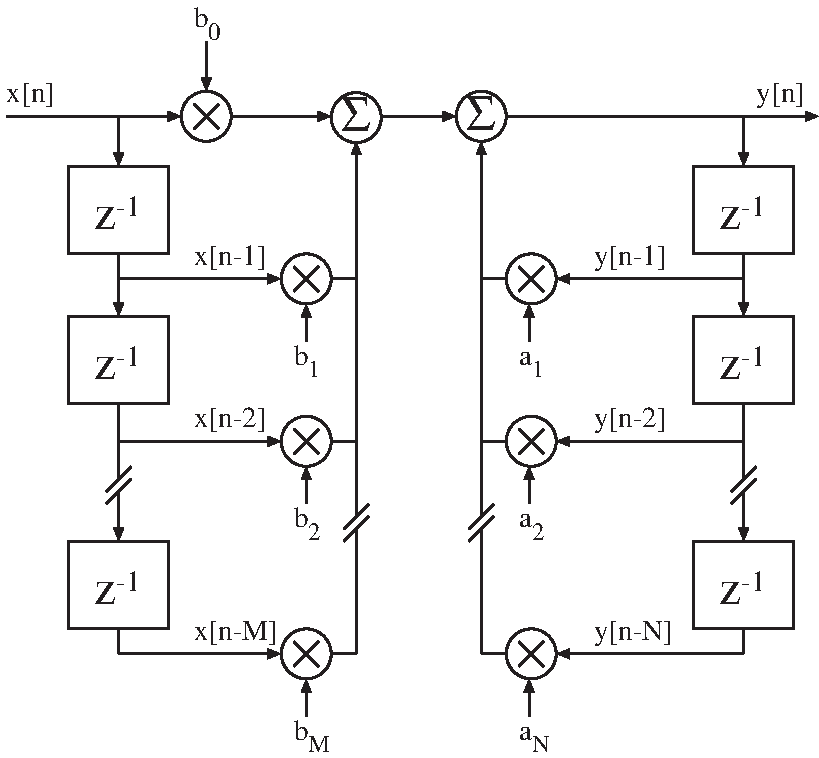
\includegraphics[width=0.5\textwidth]{ch-iir/fb-nterm-bdiag}}
\caption{Block diagram of a filter with $M$ feedforward and $N$
  feedback terms.\label{fig:fb-nterm-bdiag}}
\end{figure}

The equation for a feedback filter with $N$ feedback terms (the right
hand side of the general feedforward/feedback filter block diagram in
figure~\ref{fig:fb-nterm-bdiag}) can be written as
\begin{equation}
y[n] = x[n] - \sum_{k=1}^N a_k y[n-k]
\end{equation}
Its transfer function is 
\begin{align}
H(z) &= \frac{1}{1 + \sum_{k=1}^N a_k z^{-k}} \notag \\
     &= \frac{z^N}{z^N+\sum_{k=1}^N a_k z^{N-k}} \label{eq:manypoles}
\end{align}

Let $p_i, i=1, 2,...,N$ be its poles (the roots of the denominator
polynomial). Let's not worry about how we can get them (we know how if
we can factor the denominator polynomial, so let's assume we have
already done that).  So,~(\ref{eq:manypoles}) can be rewritten in the
form
\begin{align}
H(z) &= \frac{z^N}{(z-p_1)(z-p_2)\hdots (z-p_N)}\\
     &= \frac{z^N}{\prod_{k=1}^N(z-p_k)}\label{eq:mp-denomprod}
\end{align}
Recalling our pre-calculus, a fraction with a product of terms as
in~(\ref{eq:mp-denomprod}) can be rewritten using a partial fraction
expansion as \index{partial fraction expansion}
\begin{align}
H(z) &= \frac{A_1}{(1-p_1z^{-1})}+\frac{A_2}{(1-p_2z^{-2})}+\hdots +
\frac{A_N}{(1-p_Nz^{-N})}\\
&= \sum_{k=1}^N\frac{A_k}{(1-p_k z^{-k})}
\end{align}
Each of the terms
\begin{equation}
\frac{A_k}{(1-p_k z^{-k})}
\end{equation}
is a one-pole feedback filter. So, the complete $N$-pole filter's
output is the sum of $N$ one-pole filters' outputs. This is called a
parallel one-pole filter.
\index{filter!parallel one-pole}

\item \textbf{A one-pole feedback filter is stable if and only if its
impulse response is stable.}

Consider the unit impulse $\delta[n]$,
\begin{equation}
\delta[n] = 
\left\{\begin{array}{rl}
1 & n=0\\
0 & n>0
\end{array}\right.
\end{equation}
Any discrete input signal can be thought of as a weighted sum of
delayed unit impulses,
\begin{align}
x[n] &= \{x[0], x[1], x[2], \ldots\} \notag \\
     &= x[0]\delta[n] + x[1]\delta[n-1] + x[2]\delta[n-2] + \cdots
\end{align}
We can see that the filter's response to any signal will be stable if
and only if its response to each of these impulses is stable.

\item \textbf{An impulse response is stable if and only if its pole's
$|p|<1$.}

Equation~(\ref{eq:fb-1pexp}) tell us that the \spscript{$i$}{th}
one-pole feedback filter's impulse response is the signal with samples
\begin{equation}
1, p_i, p_i^2, p_i^3, \ldots
\end{equation}
Obviously, the impulse response is stable only when the pole's $|p_i|<1$

\item \textbf{An impulse response is neither stable nor unstable if
$|p|=1$.}
\end{enumerate}

\subsection{Resonance and Bandwidth}

\index{filter!resonance}
\emph{Resonance} is the increase in a filter's magnitude response in
the region near a pole. An example is shown in
figure~\ref{fig:fb-exp1ph90r2}. The pole is at frequency
$\hat{\omega}=\pi/2$, which is the peak of the magnitude response. The
magnitude is small when away from the pole.

One other thing mentioned before is that the peak becomes steep
when $r$ nears one. The steepness is measured by the filter's
\emph{bandwidth}.
\index{bandwidth}
Bandwidth, $B$, is defined as the width of the
filter's response (i.e., the range of frequencies) at half its maximum
power output. Bandwidth is an important measure of a filter's
performance; it indicates which frequencies are passed and which are
filtered out.

The filter's power is the square of its amplitude, so the bandwidth
can also be measured at $1/\sqrt{2}$ of its peak amplitude value.
These half power levels are denoted by
$|\mathcal{H}(\hat{\omega})|_B^2$ (the $1/\sqrt{2}$ amplitude points
written as $|\mathcal{H}(\hat{\omega})|_B$). If the peak value of
power is $|\mathcal{H}(\hat{\omega})|_p^2$ and the peak amplitude is
$|\mathcal{H}(\hat{\omega})|_p$, the bandwidth points are located at
\begin{equation}
\underbrace{|\mathcal{H}(\hat{\omega})|_B}_{\stackrel{\text{cutoff}}{_\text{amplitude}}}
  = \frac{1}{2}\underbrace{|\mathcal{H}(\hat{\omega})|_p^2}_{\stackrel{\text{peak}}{_\text{power}}}
  = \frac{1}{\sqrt{2}}\underbrace{|\mathcal{H}(\hat{\omega})|_p}_{\stackrel{\text{peak}}{_\text{amplitude}}}
\label{eq:fb-band}
\end{equation}
Since $20\log_{10}(1/\sqrt{2})=-3\mathrm{dB}$
\begin{equation}
\frac{|\mathcal{H}(\hat{\omega})|_B}{|\mathcal{H}(\hat{\omega})|_p} 
  = -3\mathrm{dB}
\end{equation}
and so the \emph{cutoff amplitude} for a filter are those for which
its output is reduced $3\mathrm{dB}$ from its peak.
\index{filter!cutoff amplitude}
\index{filter!cutoff frequency}
The values of $\hat{\omega}$ at which the filter's output is reduced
by this much define the edges of its \emph{passband} and are called
its \emph{cutoff frequencies}; they are sometimes called
its ``minus three deebee points''.
\index{filter!passband}
We will call these frequencies $\hat{\omega}_B$ in the simple case
where the passband is symmetrical and the two cutoff frequencies are
the same amount above and below the frequency at peak filter output,
$\hat{\omega}_p$.

\begin{figure}
\centerline{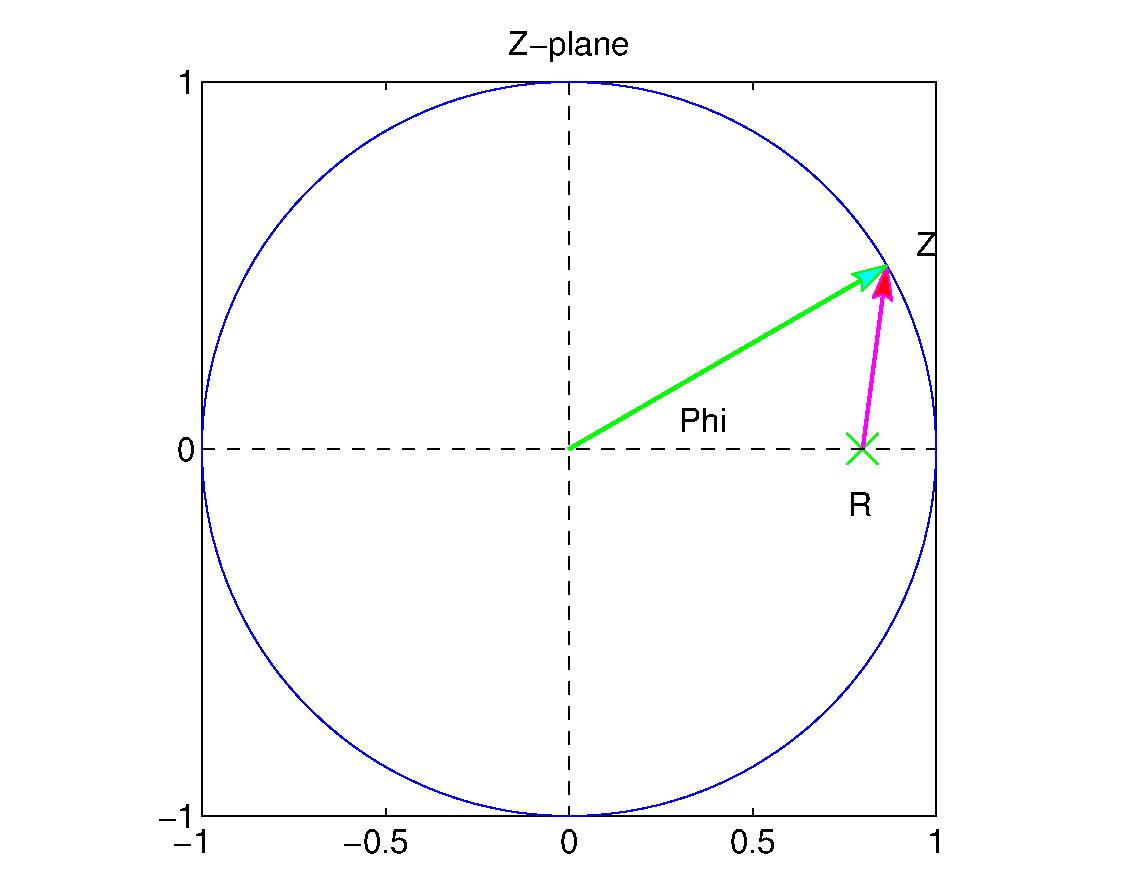
\includegraphics[height=3.5in]{ch-iir/fbexp_1p_c0_phi}}
\caption{One pole $a_1=re^{j\hat{\omega}_0}$ in z-plane. $r=R$,
$\hat{\omega}_0=0$ and $z=e^{j\hat{\omega}}$
\label{fig:fb-exp1pc0_phi}}
\end{figure}

Let's take a look at the case in which a pole is on the real axis and
no other poles are nearby; the pole is $a_1=re^{j\hat{\omega}_0}$,
$r=R$ and $\hat{\omega}_0=0$ (so $a_1=R$). A point on the unit circle
is $z=e^{j\hat{\omega}}$. This situation is illustrated in
figure~\ref{fig:fb-exp1pc0_phi}.  We know that the one pole transfer
function is
\begin{equation}
H(z)=\frac{1}{1-a_1z^{-1}}
\end{equation}
with magnitude 
\begin{equation}
|H(z)|=\left|\frac{1}{1-a_1z^{-1}}\right|
\end{equation}

Consider the inverse square of the magnitude, substituting in our
expressions for $a_1$ and $z$,
\begin{align}
\frac{1}{|\mathcal{H}(\hat{\omega})|^2}
    &= |1-R e^{j\hat{\omega}}|^2 \notag\\
    &= |1 - R\cos\hat{\omega} - jR\sin\hat{\omega}|^2 
    &&\text{(using Euler's formula)}
    \notag\\
    &= (1 - R\cos\hat{\omega})^2 + R^2\sin^2\hat{\omega} 
    &&\left(|H|^2 = \Real[\mathcal{H}]^2 + \Imag[\mathcal{H}]^2\right)
    \notag\\
    &= 1 - 2R\cos\hat{\omega} +R^2\cos^2\hat{\omega} +
       R^2\sin^2\hat{\omega} \notag\\ 
    &= 1-2R\cos\hat{\omega} + R^2
    &&\left(\cos^2\theta + \sin^2\theta = 1\right)
    \label{eq:reson-inv-mag2}
\end{align}
The peak of $|\mathcal{H}(\hat{\omega})|^2$ should be the value of
angle $\hat{\omega}_p=\hat{\omega}$ that makes
$1/|\mathcal{H}(\hat{\omega})|^2=1-2R\cos\hat{\omega} + R^2$ minimum,
that is when $\hat{\omega}=0$. The power at this peak is determined by
substituting $\hat{\omega}=0$ into equation~(\ref{eq:reson-inv-mag2})
and taking its reciprocal:
\begin{equation}
|\mathcal{H}(\hat{\omega})|^2_p=\frac{1}{(1-R)^2}
\end{equation}
According to equation (\ref{eq:fb-band}), 
\begin{equation}
|\mathcal{H}(\hat{\omega})|_B
  =\frac{1}{2}|\mathcal{H}(\hat{\omega})|^2_p=\frac{1}{2(1-R)^2}
\end{equation}
The corresponding $\hat{\omega}_B$ can be obtained by substituting
$|\mathcal{H}(\hat{\omega})|_B$ for $|\mathcal{H}(\hat{\omega})|$ in
equation~(\ref{eq:reson-inv-mag2}) and solving for frequency:
\begin{align}
2(1-R)^2 &= 1-2R\cos\hat{\omega_B}+R^2 \label{eq:fb-band2a}\\
\cos\hat{\omega}_B &= 2-\frac{1}{2}\left(R+\frac{1}{R}\right)
\label{eq:fb-band2b}
\end{align} 

The filter's bandwidth is the span $[-\hat{\omega}_B, \hat{\omega}_B]$
--- a distance of $2\hat{\omega}_B$.  When $R$ is close to one, we can
express $R$ as a small amount $\epsilon$ less than one:
$R=1-\epsilon$. We can then take advantage of the expansions:
\begin{equation}
\frac{1}{R}=\frac{1}{1-\epsilon}=1+\epsilon+\epsilon^2+\epsilon^3+\cdots
\end{equation}
and
\begin{equation}
\cos\epsilon=1-\frac{\epsilon^2}{2!}+\frac{\epsilon^4}{4!}+\cdots
\end{equation}
So, from~(\ref{eq:fb-band2b}),
\begin{align}
\cos\hat{\omega}_B &= 2-\frac{1}{2}[\underbrace{(1-\epsilon)}_{R} +
            \underbrace{(1+\epsilon+\epsilon^2+\epsilon^3+\cdots)}_{\frac{1}{R}}]
              \notag\\
   &= 1-\frac{\epsilon^2}{2}-O(\epsilon^3) \notag\\
   &\approx \cos\epsilon
\end{align} 
(where $O(\epsilon^3)$ is shorthand for terms in the expansion of
order $\epsilon^3$ or higher).  Therefore,
$\hat{\omega}_B\approx\epsilon$.  So, when $R$ is close to the unit
circle,
\begin{equation}
B = 2\hat{\omega}_B \approx 2\epsilon =2(1-R)
\end{equation}
or 
\begin{equation}
R \approx 1-B/2
\label{eq:calc-bw}
\end{equation}
If we want a low-pass filter with a particular bandwidth,
equation~(\ref{eq:calc-bw}) gives us a way to determine its pole
location.

\problemset{
\subsubsection{Self-Test Exercises}

See~\ref{sc:ch4ex} \#\ref{it:ch4ex1}--\ref{it:ch4ex2} for answers.

\begin{enumerate}
\item Derive equation~(\ref{eq:fb-band2b})
  from~(\ref{eq:fb-band2a}).
\item In the situation where the sampling rate is 44,100Hz and the
  desired bandwidth is 20Hz, $R$ in~(\ref{eq:calc-bw}) is 0.998575.
  Solve for $R$ the situation where the desired bandwidth is 200Hz. Is
  it true that when $R$ is far away from one, $B$ grows large?
\end{enumerate}}

\section{Mixing Feedback and Feedforward Filters}

We have now seen feedforward filters with zeros in the transfer
function and feedback filters with poles. Zeros suppress frequency
components and poles enhance them.  Quite often, we want to combine
poles and zeros to improve the filter's features, such as the flatness
of the passband and the abruptness with which its response transitions
between the passband and the stop band.  Generally, the transfer
function of a filter with block diagram in
figure~\ref{fig:fb-nterm-bdiag} can written as
\begin{equation}
H(z)=\frac{b_0+b_1z^{-1}+\cdots+b_Mz^{-M}}{1+a_1z^{-1}+\cdots+a_Nz^{-N}}
\label{eq:gen-xfer}
\end{equation}
and the filter is  
\begin{equation}
y[n] = \underbrace{b_0x[n] + b_1x[n-1] + \cdots +
      b_Mx[n-M]}_{\text{feedforward terms}}
      - 
      \underbrace{a_1y[n-1] - \cdots - a_ny[n-N]}_{\text{feedback terms}}
\label{eq:gen-impl}
\end{equation}

Depending on the coefficients $\{b_k\}$ and $\{a_\ell\}$, the
filter will show different features. Some of these features have
proven so useful that these forms of~(\ref{eq:gen-xfer}) have acquired
special names, such as elliptic, Butterworth, etc (usually, based on
the form of the numerator and/or denominator polynomial).

\section{Implementation}

Just as in chapter~\ref{ch:filt-intro}, feedback filters have their
delays implemented with queues which are ``circular arrays''.
However, there are two additional complications that we must deal
with: complex poles and accuracy of numerical computation.

\subsection{Avoiding Complex Numbers}

In principle, there is no reason that we couldn't perform all our
computations using complex numbers and just output the real part of
the result as the filtered signal.  However, we often want to perform
filtering in real time, and so would like to avoid any unnecessary
computation. A cute trick allows us to eliminate the need for complex
numbers.

\emph{Remember that all complex poles will appear in conjugate pairs.}
Since each pole is a root of a polynomial, that means that the
denominator of the filter's transfer function will have even degree
(excepting the real-valued poles, of course), and when it is factored
the conjugate pairs $(z_i,z_i^*)$ will appear as $(z-z_i)(z-z_i^*)$.
If we multiply this out, we get $z^2 - 2\Real[z_i] z +|z_i|^2$. In
other words, the imaginary parts of poles cancel each other out.
Since we're already using $b_k$ for the feedforward coefficients and
$a_\ell$ for the feedback ones in the filter equation, let's set $c_i
= -2\Real[z_i]$ and $d_i = |z_i|^2$.  If the transfer function's
denominator is of order $N$ ($N$ even), then we can multiply out the
polynomials for each complex conjugate pair and rewrite the
denominator as the product of $N/2$ second-order polynomials
\begin{equation}
(z^2+c_0z+d_0)(z^2+c_1z+d_1)\cdots (z^2+c_{N/2-1}z+d_{N/2-1})
\end{equation}
with no need for complex arithmetic.  We've done this before
symbolically, using Euler's formula to eliminate the imaginary part of
a complex conjugate pair. The point here is that, since complex poles
always appear in conjugate pairs, we can do this with even quite
complicated filters to eliminate the need for performing complex
arithmetic or processing complex numbers --- a significant
optimization.

\subsection{Limitations of Numerical Accuracy}

When we talk of the mathematics of filters, we assume that numbers
have infinite precision.  Unfortunately, this is not the case for
computer implementation.  These days, computers (including digital
signal processors) typically use either 32 or 64 bits to represent
numbers (be they fixed or floating point).  That may seem like a great
deal of precision, but it is unfortunately not uncommon for
intermediate results in numerical computation to require many more
bits to retain needed precision.  There are a number of ways this can
happen, but one is where a computation is performed iteratively, so
that a long chain of operations is applied to inputs before they
become outputs. At each step of this chain, the result has limited
precision. In other words, the number we get is not exactly correct
--- in general, it can't be, since we don't have infinite precision.

This loss of precision can mount rapidly, eventually destroying the
result. We can think of this limited precision as an \emph{error}. If
the input is from a 16-bit A/D, for example, and we assume it does its
conversion absolutely accurately to the smallest bit (which, as you
have seen in chapter~\ref{ch:computer-signals} and will revisit in
chapter~\ref{ch:compression}, is probably not realistic), then that's
around $\log_{10} 2^{16} \approx 5$ decimal digits from the A/D, to be
generous. Each arithmetic operation we perform, regardless of the
number of bits we use, can have the undesirable effect of decreasing
the number of digits of precision we have.  Sums of approximate values
have errors which are the sums of their addends' errors.
Multiplication tends to magnify errors. Let's see this with a simple
example.

\paragraph{Example~4}
Consider the following two recurrence relations for computing the
series $\{x[n]\} = \{1/3^n\}$ ($n = 0, 1, 2, \ldots$):
\begin{align}
x'[n]  &= \frac{1}{3} x'[n-1] \label{eq:series-direct} \\
x''[n] &= \frac{10}{3} x''[n-1] - x''[n-2]
\label{eq:series-twoterms}
\end{align}
Both of these equations are mathematically ``correct''. \emph{They
also look like the expressions we use for our filters.}  Yet, they
yield very different results because of loss of significance.  Let's
use an initial value of $x'[0] = 0.99996$ for~(\ref{eq:series-direct})
and initial values of $x''[0]=1$ and $x''[1]=0.33332$
for~(\ref{eq:series-twoterms}). This is an initial error of 0.00004
for $x'[0]$ and $0.00001\bar{3}$ for $x''[1]$. I'll use MATLAB to
compute the first ten terms in each sequence with double-precision
accuracy for each calculation.  The MATLAB code is
\index{MATLAB code!numerical error|(}

\begin{small}
\begin{verbatim}
% significance.m
% 2/22/02 MDS
% Examine how error grows in an iterative computation
stdout = 1;

% This isn't efficient, but it is straightforward

% Values of n for computation
n = [0:10];

% Series 1: the real McCoy
x = 1./3.^n;

% Series 2: x'[n] = 1/3 x'[n-1]
xp = 0.99996;

for n = [1:10],
  xp(n+1) = 1/3 * xp(n);  % Remember, MATLAB indices start at 1, not 0
end;

% Series 3: x''[n] = 10/3 x''[n-1] - x''[n-2]
xpp = [1 0.33332];

for n = [2:10],
  xpp(n+1) = 10/3 * xpp(n) - xpp(n-1);
end;

% Print out the results
fprintf(stdout, ' n          x[n]            x''[n]           x''''[n]\n');
for n = [0:10],
  fprintf(stdout, '%2.1d\t%12.10f\t%12.10f\t%12.10f\n', ...
          n, x(n+1), xp(n+1), xpp(n+1));
end;
\end{verbatim}
\end{small}

The output this script produces is:
\begin{verbatim}
 n          x[n]            x'[n]           x''[n]
 0      1.0000000000    0.9999600000    1.0000000000
 1      0.3333333333    0.3333200000    0.3333200000
 2      0.1111111111    0.1111066667    0.1110666667
 3      0.0370370370    0.0370355556    0.0369022222
 4      0.0123456790    0.0123451852    0.0119407407
 5      0.0041152263    0.0041150617    0.0029002469
 6      0.0013717421    0.0013716872    -0.0022732510
 7      0.0004572474    0.0004572291    -0.0104777503
 8      0.0001524158    0.0001524097    -0.0326525834
 9      0.0000508053    0.0000508032    -0.0983641945
10      0.0000169351    0.0000169344    -0.2952280648
\end{verbatim}
\index{MATLAB code!numerical error|)}

The first column is accurate to the full precision of IEEE floating
point (that is, the computation is that accurate; the output was
limited to ten decimal places).  The second column's error is
\emph{stable}: it decreases in an exponential manner, and the value
for $x'[10]$ is within $7 \times 10^{-10}$ of the actual value. The
third column's error is \emph{unstable}: it increases exponentially.

Couple this with the need for precise pole placement, and you
can see that we need to be careful about our implementations. We saw
in this chapter's section on combining feedforward and feedback
filters the general transfer function for a filter~(\ref{eq:gen-xfer})
and its direct implementation~(\ref{eq:gen-impl}), which involved
$M$ delayed values of $x$ and $N$ delayed values of $y$.

\index{filter!cascade}
However, it is better to implement such a digital filter as a cascade
of second-order ones, by factoring the numerator and denominator
(which should be ``easy,'' since we know the locations of the poles
and zeros) and multiplying out terms with complex conjugate pairs as
described in the previous section. The resultant fraction will have
numerator and denominator which are each a product of second-order
polynomials.  Each ratio of second-order polynomials is a subfilter,
which can be implemented by a simple update equation. If we take the
output of one subfilter and present it as the input of the next, the
output of the last subfilter will be equivalent to the output of the
entire original filter (we saw this cascade of filters in
chapter~\ref{ch:filt-intro}). Note that, though each filter has a very
short (two step) queue, the series combination produces what amounts
to a longer overall queue. In practical applications, this shouldn't
be much of a computational penalty.

\section{Problems}


\section{Further Reading}

\begin{itemize}
\item James H McClellan, Ronald W. Schafer, and Mark A. Yoder,
  \textit{DSP First: A Multimedia Approach}, Prentice Hall, 1998,
  chapter 8 (\S 8.1--8.6, 8.8).
\end{itemize}


% LocalWords:  feedforward phasor reson
